\newpage
\section{Introduction}

Cavity electrodynamics\cite{Haroche} is the study of light confined inside an optical resonater and, in the case of this project, quantized as a basis of harmonic oscillator modes\cite{Sakurai}. The quantization of the electromagnetic (EM) field inside an optical cavity has been, and continues to be, paramount in the advancement of fields such as optical communication, quantum optics, photonics, sensing, optomechanics\cite{Monsel,Sankey}, etc. The ability to enhance mode selection of a coherent light source allows for an increase in control of a given system, and highly resolved measurements\cite{Vahala}.

Many different types of resonators and materials have been utilized for cavity electrodynamics, e.g. beams, drums, photonic crystals and membranes\cite{Thompson,Jayich}. The latter is here of specific interest, as low mass \emph{Silicon Nitride (SiN)} membranes\cite{Wilson} have proven to posses low losses in the visible- and infrared spectral ranges\cite{Land}, and has furthermore been shown to have excellent mechanical properties\cite{Seis,Cupertino}. Examples of applications of $SiN$ membranes as mechanical resonators used in cavity electrodynamics are as transducers between optical and microwave fields in telecommunication\cite{Bagci,Andrews} and in sensing for accelerometry\cite{Chowdhury,Manley}, thermometry\cite{Ferreiro-Vila,Zhang,Nair_thesis} and pressure sensing\cite{Naserbakht,Al-Sumaidae,Hornig,Salimi}. 

However, while $SiN$ membranes are great mechanical resonators, they typically display relatively low reflectivities of $\sim 10\%$ - $35\%$. That is when only the bare membrane is considered. In order to preserve the quality of the mechanical properties along with the low mass, while achieving higher values for the reflectivity, the membranes are patterned with periodic sub-wavelength, 1- or 2-dimensional, photonic crystal structures\cite{Kemiktarak,Kemiktarak2,Bui,Norte,Reinhardt,Chen,Zhou}. In the past decade, tremendous strides have been made in the field of micro- and nano-fabrication methods, and patterned membranes with a record reflectivity of as high as $\sim 99.9998\%$ have been reported\cite{Xu,Sang,Enzian}.

The type of patterned membrane considered for this project is a 1-dimensional sub-wavelength grating with optical properties well-described by the theory presented by Fan and Joannopoulos \cite{Fan-Joannopoulos-guided-mode-resonance,Fan-Joannopoulos-fano-resonance}. It is thus said to act as so-called \emph{Fano mirrors} with transmission and reflection coefficients dependent on the incident wavelength. The wavelength-dependence gives rise to a \emph{guided-mode} resonance which can bu utilized in the designing of optical \emph{Fano} cavities with spectra showcasing ultra-narrow linewidth resonance peaks\cite{Mitra,Manjeshwar}. By tuning the cavity mode and incoming EM-field to match the guided-mode, one can resolve structures with a linewidth in the low picometer regime for cavity lengths down to a few microns. 

In previous work, the single Fano cavity has been realized and characterized, consisting of a broadband mirror and a Fano mirror in a plane-plane configuration. The Fano cavity have proved to produce ultra-narrow linewidth resonance spectra for very short cavity lengths, while still maintaining a high radiation pressure and thus mechanical Q-factor. This makes them an excellent candidate as subjects for optomechanical experiments and corresponding sensing applications. 

In this project we propose the \emph{double Fano cavity} as an expansion of the theory presented for the single Fano cavity by Mitra et al. in \cite{Mitra}. The double Fano cavity consists of two Fano mirrors with each their wavelength-dependent set of optical coefficients and will thus, theoretically, produce an even narrower resonance profile than the \emph{single} Fano cavity. Figure \ref{fig:all_cavities_sketch} shows schematics for all three aforementioned optical cavities, namely the broadband cavity (\ref{fig:broadband_cavity_sketch}), single Fano cavity (\ref{fig:single_fano_cavity_sketch}) and double Fano cavity (\ref{fig:double_fano_cavity_sketch}), where $t_g, r_g$ refers to transmission- and reflection coefficients of a Fano mirror, and $t_m, r_m$ are the ones for a broadband mirror.

\begin{figure}[h!]
    \centering
    \begin{subfigure}[b]{0.3\textwidth}
        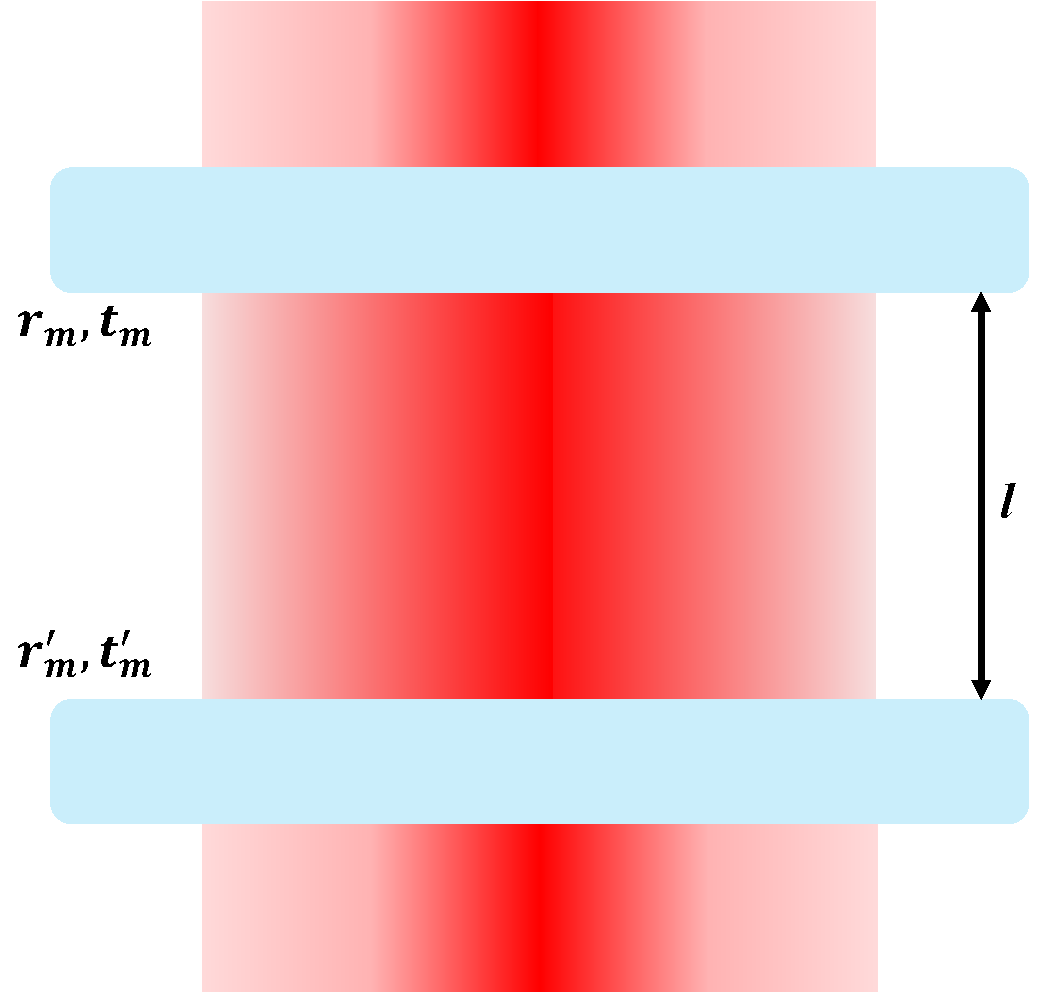
\includegraphics[width=\textwidth]{figures/broadband_sketch.pdf}
        \caption{Broadband cavity.}
        \label{fig:broadband_cavity_sketch}
    \end{subfigure}
    \hfill
    \begin{subfigure}[b]{0.3\textwidth}
        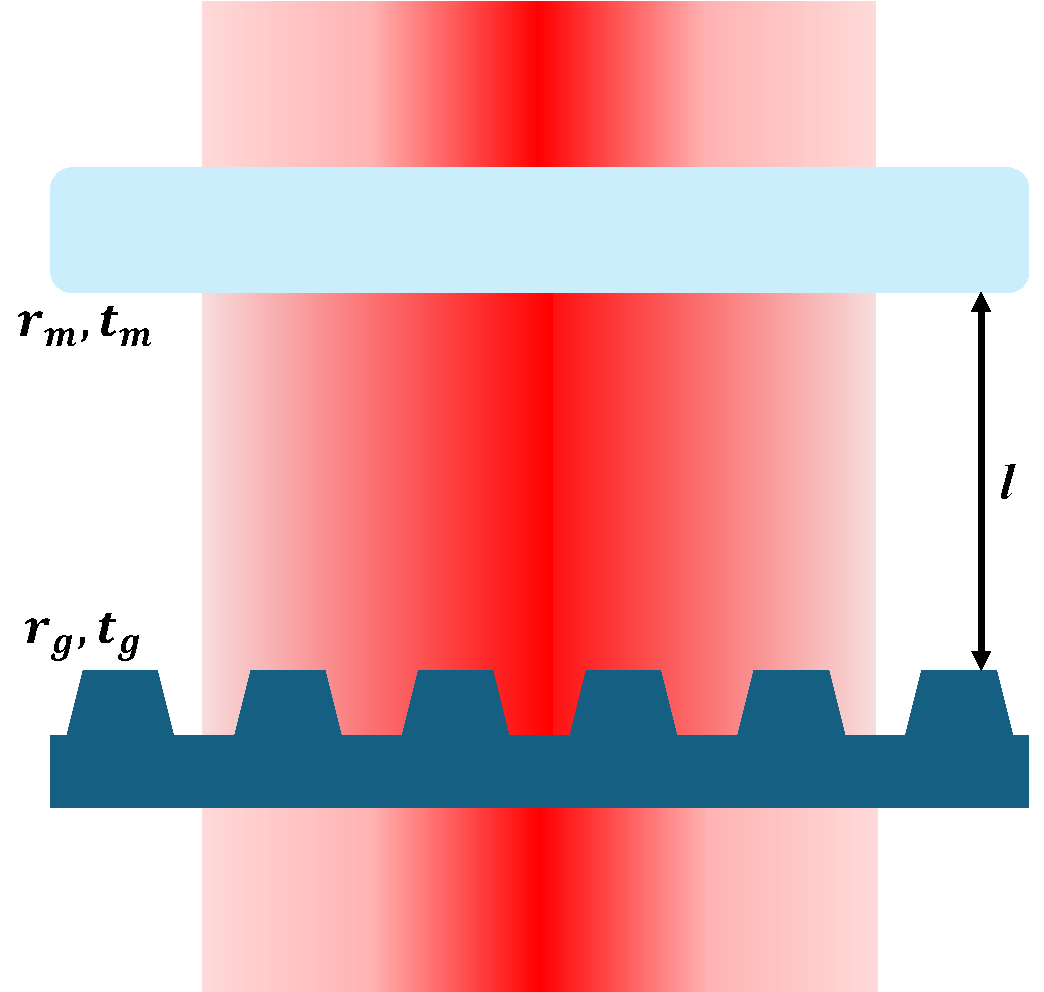
\includegraphics[width=\textwidth]{figures/single_fano_sketch.pdf}
        \caption{Single Fano cavity.}
        \label{fig:single_fano_cavity_sketch}
    \end{subfigure}
    \hfill
    \begin{subfigure}[b]{0.3\textwidth}
        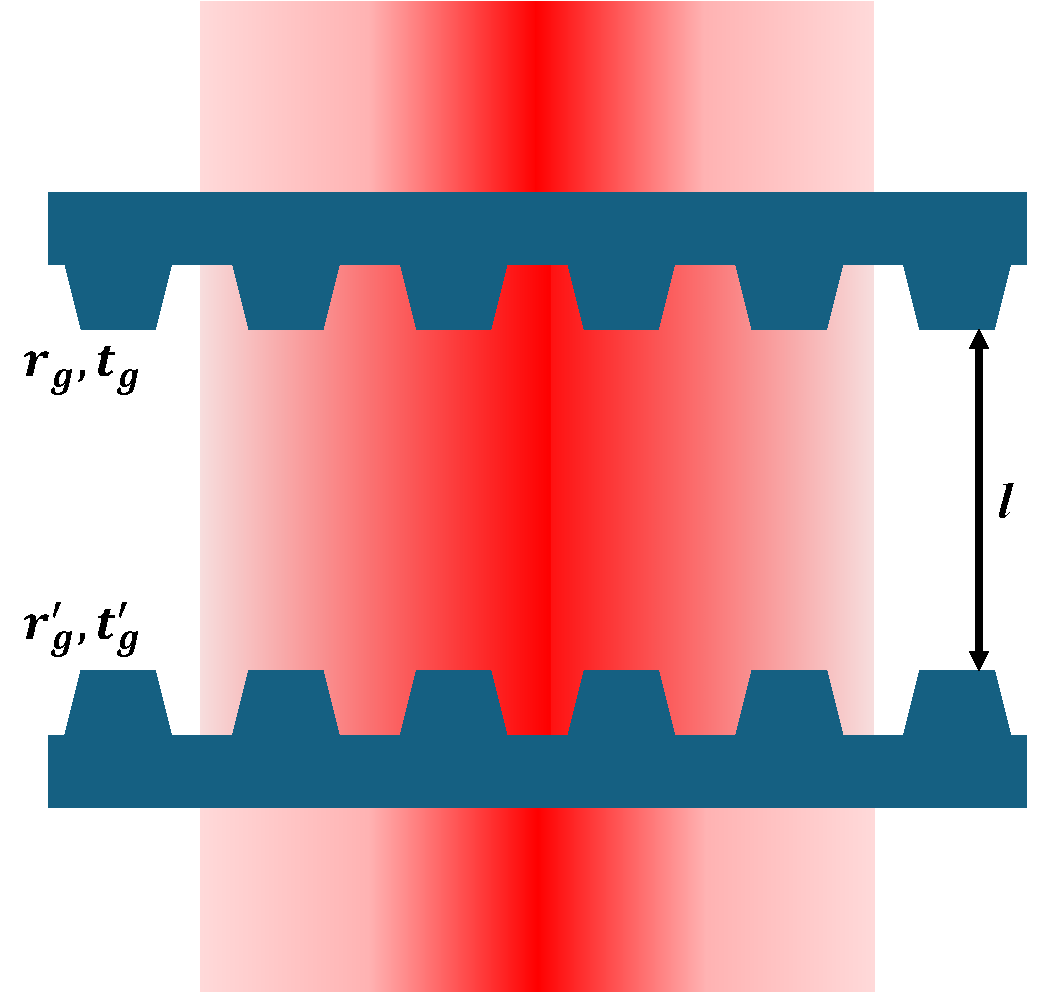
\includegraphics[width=\textwidth]{figures/double_fano_sketch.pdf}
        \caption{Double Fano cavity.}
        \label{fig:double_fano_cavity_sketch}
    \end{subfigure}
    \caption{}
    \label{fig:all_cavities_sketch}
\end{figure}

In this thesis I will present the theory of the sub-wavelength grating, i.e. Fano mirrors, and of the single- and double Fano cavities. I will show extensive simulations run for the transmission spectra of the double Fano cavity as a part of my investigations in order to map the on- and off-resonance behaviour as functions of various physical parameters. I will expand in detail on the experimental methods and techniques used in order to realize said theory and outline obstacles faced in that process. Finally I will present the results of my project and compare these with analytical predictions and discuss shortcomings and sources of error and noise of the setup and methods used. I will end by briefly dicussing the possible outlook of future projects regarding the double Fano cavity and the field of cavity electrodynamics generally in the light of my findings. 